
\section{Experiments}
\label{sec:experiments}
\looseness-1We first compare our method against reachability baselines and then evaluate it on reachability analysis for a unicycle (3D), planar quadcopter (6D), 3D quadcopter (12D), MuJoCo \citep{todorov2012mujoco} hopper (11D), and MuJoCo swimmer (28D). All experiments are run on a desktop with an Intel i9-14900K CPU, 64\,GB RAM, and an NVIDIA RTX 4090 GPU. For the MuJoCo examples, we set the planner $P$ to be an expert PPO \citep{schulman2017proximalpolicyoptimizationalgorithms} policy; for the other systems, we use a trajectory optimizer on the analytical dynamics to serve as $P$. We report four key metrics: (i) \textit{reachability runtime} (s), where lower is better; (ii) \textit{average log-volume of reachable sets}, where lower indicates less conservativeness; (iii) \textit{safety rate over rollouts}, where higher is better; and (iv) \textit{coverage variability for CP-based verification}, where lower Beta-posterior variance of empirical coverage across calibration sizes indicates more stable coverage. Some metrics apply only to specific baselines (e.g., safety filters report safety rate only). Comprehensive results are presented in Table~\ref{tab:result_tab}.

\paragraph{Baselines}
\looseness-1We select baselines to highlight four gaps in data-driven reachability. (i) Learned reachability estimators \citep{deepreach} lack overapproximation guarantees, motivating formal NN verification. (ii) Existing hybrid CP-NNV (CP-NNV) \citep{cp_baseline} methods struggle to scale to high-dimensional, nonlinear dynamics and long horizons, motivating the Koopman lift. (iii) Pure CP-based reachability approaches \citep{cp_survey} suffer coverage degradation as calibration data or sample budgets shrink, motivating sample-efficient reachability analysis that remains reliable under limited data. (iv) Pure NNV-based RSOA computation \citep{sage-mp} provides deterministic guarantees but can be slow, motivating fast Koopman-based linear reachability.

\noindent\textit{\myuline{Unsafe behavior from learned reachability estimators.} } Under unicycle dynamics \eqref{eq:unicycle}, a value-function-based safety filter \citep{deepreach} -- an approximate reachability method -- fails to consistently enforce reach-avoid safety, with only 70\% of 250 rollouts satisfying the constraint (Fig. \ref{fig:deepreach}). Because the learned value function is an approximate neural PDE solution, small errors in the value and its gradient can cause safety violations, and the method lacks formal guarantees. In contrast, our method provides calibrated probabilistic guarantees that the closed-loop system remains in the CKRS computed via \eqref{eq:conformal_inflation} (100\% in our experiments) while preserving goal-reaching.

\noindent \textit{\myuline{Pure CP based verification.} }
Because our learned Koopman lift closely matches the training dynamics, the resulting KRS are already tight; conformalization then serves only to absorb the small residual model error. We compare to a pure SNSA baseline \citep{cp_survey}, which aggregates all heterogeneous trajectory and state errors into a single nonconformity score. As the horizon or state dimension grows, this forces the baseline to either inflate its sets or require much larger calibration sets to achieve the target $\delta$, causing it to suffer from slow convergence to the target coverage level. At practical data budgets (e.g., 1000 samples), a large coverage variance remains, e.g., as much as 5\% under-coverage of the true system trajectories (Fig. \ref{fig:pure_cp}), which can compromise system safety. In contrast, our method attains $100\%$ empirical coverage across all tested calibration set sizes, avoiding this variance-data trade-off and achieving target coverage with far fewer samples.

\begin{figure}[ht]
    \centering
    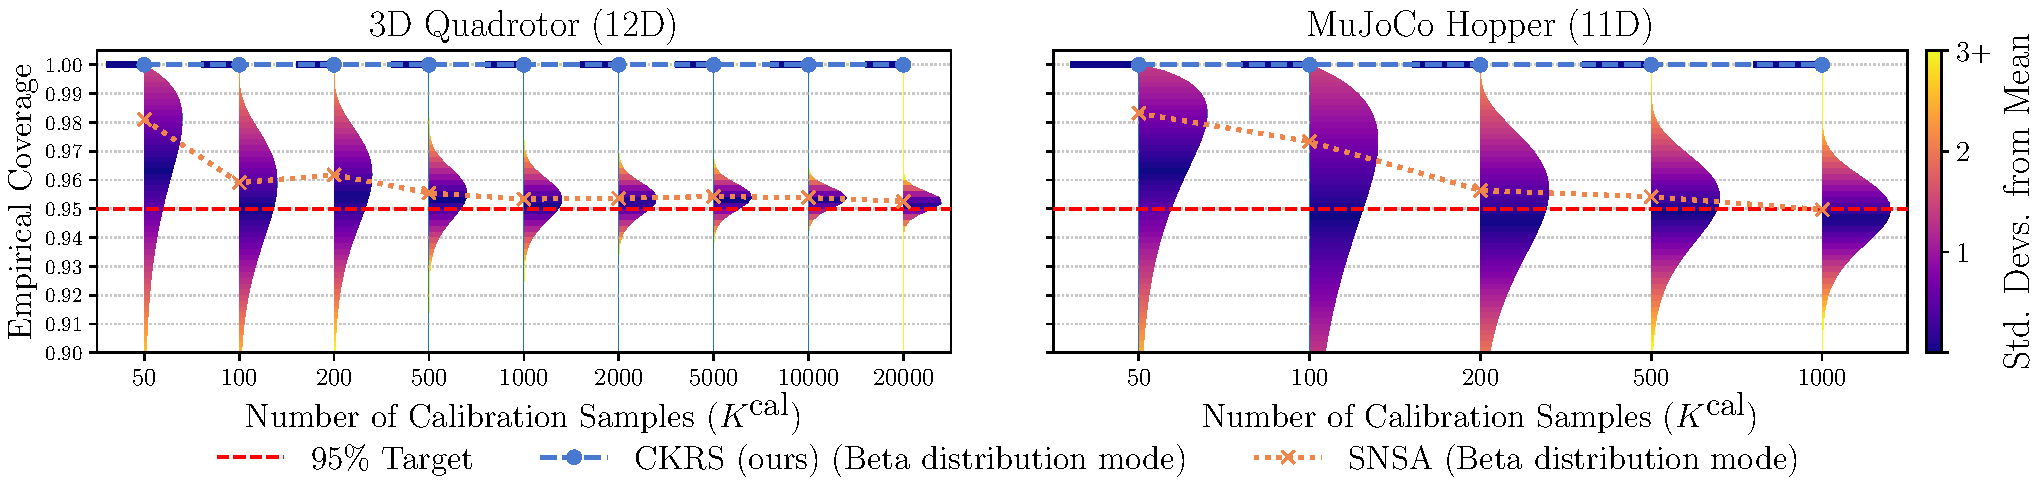
\includegraphics[width=\linewidth]{img/pure_cp_base/pure_cp_base_combined_v2.pdf}
    \caption{\looseness-1To visualize empirical reachable set coverage, we compute Beta posteriors for the SNSA baseline and ScaRe-Kro on the 3D quadcopter (left) and Hopper (right). The dotted lines indicate the mode of the Beta posterior. For SNSA, coverage rate slowly converges to the target $1-\delta$ as calibration dataset size increases, whereas ScaRe-Kro maintains $100\%$ coverage even for small $K^\textrm{cal}$.}
    \label{fig:pure_cp}
\end{figure}

\noindent \textit{\myuline{Hybrid Reachability methods (CP+NNV).} }
\looseness-1For a 3D quadcopter \eqref{eq:3D_Quad_dyn}, we compare with a hybrid data-driven/NNV reachability method \citep{cp_baseline} (denoted CP-NNV), that computes an RSOA by applying NNV on a learned NN trajectory predictor and using CP to bound RSOA underapproximation error induced by learning error. As shown in Fig.~\ref{fig:cpnnv}, CP-NNV yields much larger reachable sets (avg. log volume: -23.35), especially in attitude and velocity. This reflects difficulties in scaling NNV and CP to high-dimensional state spaces and long horizons, which we address with Koopman operators. Our method produces tighter RSOAs (avg. log volume: -40.66) while maintaining coverage, improving scalability with horizon and reducing conservativeness.

\noindent \textit{\myuline{Pure NNV Reachability.} }
On a unicycle model, we compare with our prior work \citep{sage-mp}, which used NNV tools for one-shot RSOA computation, requiring $51.95$s and achieving an average log-volume of $-3.98$. In contrast, our method computes the RSOA in $0.32$s with a log-volume of $-11.54$ (Table \ref{tab:result_tab}). This highlights that our method is much faster and also reduces conservativeness.

\begingroup
\setlength{\textfloatsep}{4pt}
\setlength{\intextsep}{4pt}
\setlength{\floatsep}{4pt}
\setlength{\abovecaptionskip}{2pt}
\setlength{\belowcaptionskip}{0pt}
\renewcommand{\arraystretch}{0.5}   % row height
\setlength{\tabcolsep}{3pt}         % column padding
\setlength{\aboverulesep}{0pt}
\setlength{\belowrulesep}{0pt}
\setlength{\cmidrulesep}{2pt}

\newcommand{\thdr}[1]{\smash[b]{\shortstack{#1}}}

\begin{table}[!t]
\centering
\scriptsize
\caption{Numerical RSOA results for SCaRe-Kro on unicycle, quadcopters and MuJoCo models.}
\label{tab:result_tab}
\begin{tabular}{lcccccccccc}
\toprule
\textbf{Experiment} &
\textbf{\thdr{System\\dimension}} &
\textbf{\thdr{Time\\steps}} &
\textbf{\thdr{Confidence\\Level\\$(1-\delta)$}} &
\textbf{\thdr{CP\\time}} &
\textbf{\thdr{KRS\\time}} &
\textbf{\thdr{Total\\time\\(online)}} &
\textbf{\thdr{Avg. Log\\volume\\(online)}} &
\textbf{\thdr{Avg. Log\\volume\\(offline)}} &
\textbf{\thdr{Calibration\\dataset\\size}} &
\textbf{\thdr{Empirical\\coverage}} \\
\midrule
Unicycle & 3  & $100$ & $99.0\%$ & $0.038$s & $0.277$s & $0.315$s & $-11.543$ & $-8.690$ & $100$  &  $100\%$\\
2D Quad  & 6  & $100$ & $99.0\%$ & $0.055$s & $0.349$s & $0.404$s & $-21.491$ & $-5.333$  & $100$ & $100\%$ \\
3D Quad  & 12 & $200$ & $99.0\%$ & $0.175$s & $0.500$s & $0.675$s & $-42.954$ & $-35.275$ & $100$ & $100\%$ \\
Hopper   & 11 & $225$ & $99.0\%$ & $10.597$s & $0.387$s & $10.983$s & $-4.969$ & $-1.806$ & $100$ & $100\%$ \\
Swimmer  & 28 & $400$ & $95.0\%$ & $20.818$s & $0.593$s & $21.411$s & $32.595$ & $42.617$ & $100$ & $99.5\%$ \\
\bottomrule
\end{tabular}
\end{table}


\endgroup

\paragraph{Unicycle}
\looseness-1
We evaluate on CKRS computations on a unicycle model \eqref{eq:unicycle}, where $\enc$ and $\dec$ have 3 hidden layers with 128 neurons each, and $z \in \mathbb{R}^{10}$. As shown in Fig.~\ref{fig:car}, the certified reachable sets verify both safety and goal attainment. Full metrics are in Table~\ref{tab:result_tab}. We view this benchmark as a sanity check on a simple system, paving the way for more substantive scalability results.

\paragraph{Planar Quadcopter}
\looseness-1We evaluate a 6-state planar quadcopter \eqref{eq:2dquad} navigating around a circular obstacle for $T=100$. Here, $\enc$ and $\dec$ have 3 hidden layers with 128 neurons each, and $z \in \mathbb{R}^{24}$. We visualize offline-calibrated CKRSs for multiple reference trajectories in Fig.~\ref{fig:2d_quad}; metrics are in Table~\ref{tab:result_tab}. An NNV-only baseline \citep{sage-mp} required $59.85\,\mathrm{s}$ and achieved an average log-volume of $-18.709$. Overall, these results support our claim of reduced RSOA conservativeness. 

\paragraph{3D Quadcopter}
\looseness-1
\label{sec:3dquad}
We evaluate an analytical 12-state quadcopter \eqref{eq:3D_Quad_dyn} \citep{sabatino2015quadrotor} navigating around a $1\,\mathrm{m}$ radius obstacle for $T=200$. Here, $\enc$ and $\dec$ have 3 hidden layers with 128 neurons each, and $z \in \mathbb{R}^{24}$. The computed CKRS (Fig.~\ref{fig:3d_quad}) verifies safety and goal reaching; metrics are in Table~\ref{tab:result_tab}. To show that the offline CP inflation generalizes across controllers, we compute the CKRS for two references (Fig. \ref{fig:3d_quad}, one orange, one blue) using the same offline-calibrated bounds; we visualize additional CKRSs in Fig. \ref{fig:3d_quad_alt}. An NNV-only baseline \citep{sage-mp} is much slower and more conservative, requiring $2153.45\,\mathrm{s}$ with an average log-volume of $-30.32$. Overall, these results show our method's efficiency, tightness, and offline CP generalization for high-dimensional systems.

\begin{figure}[ht]
    \centering
    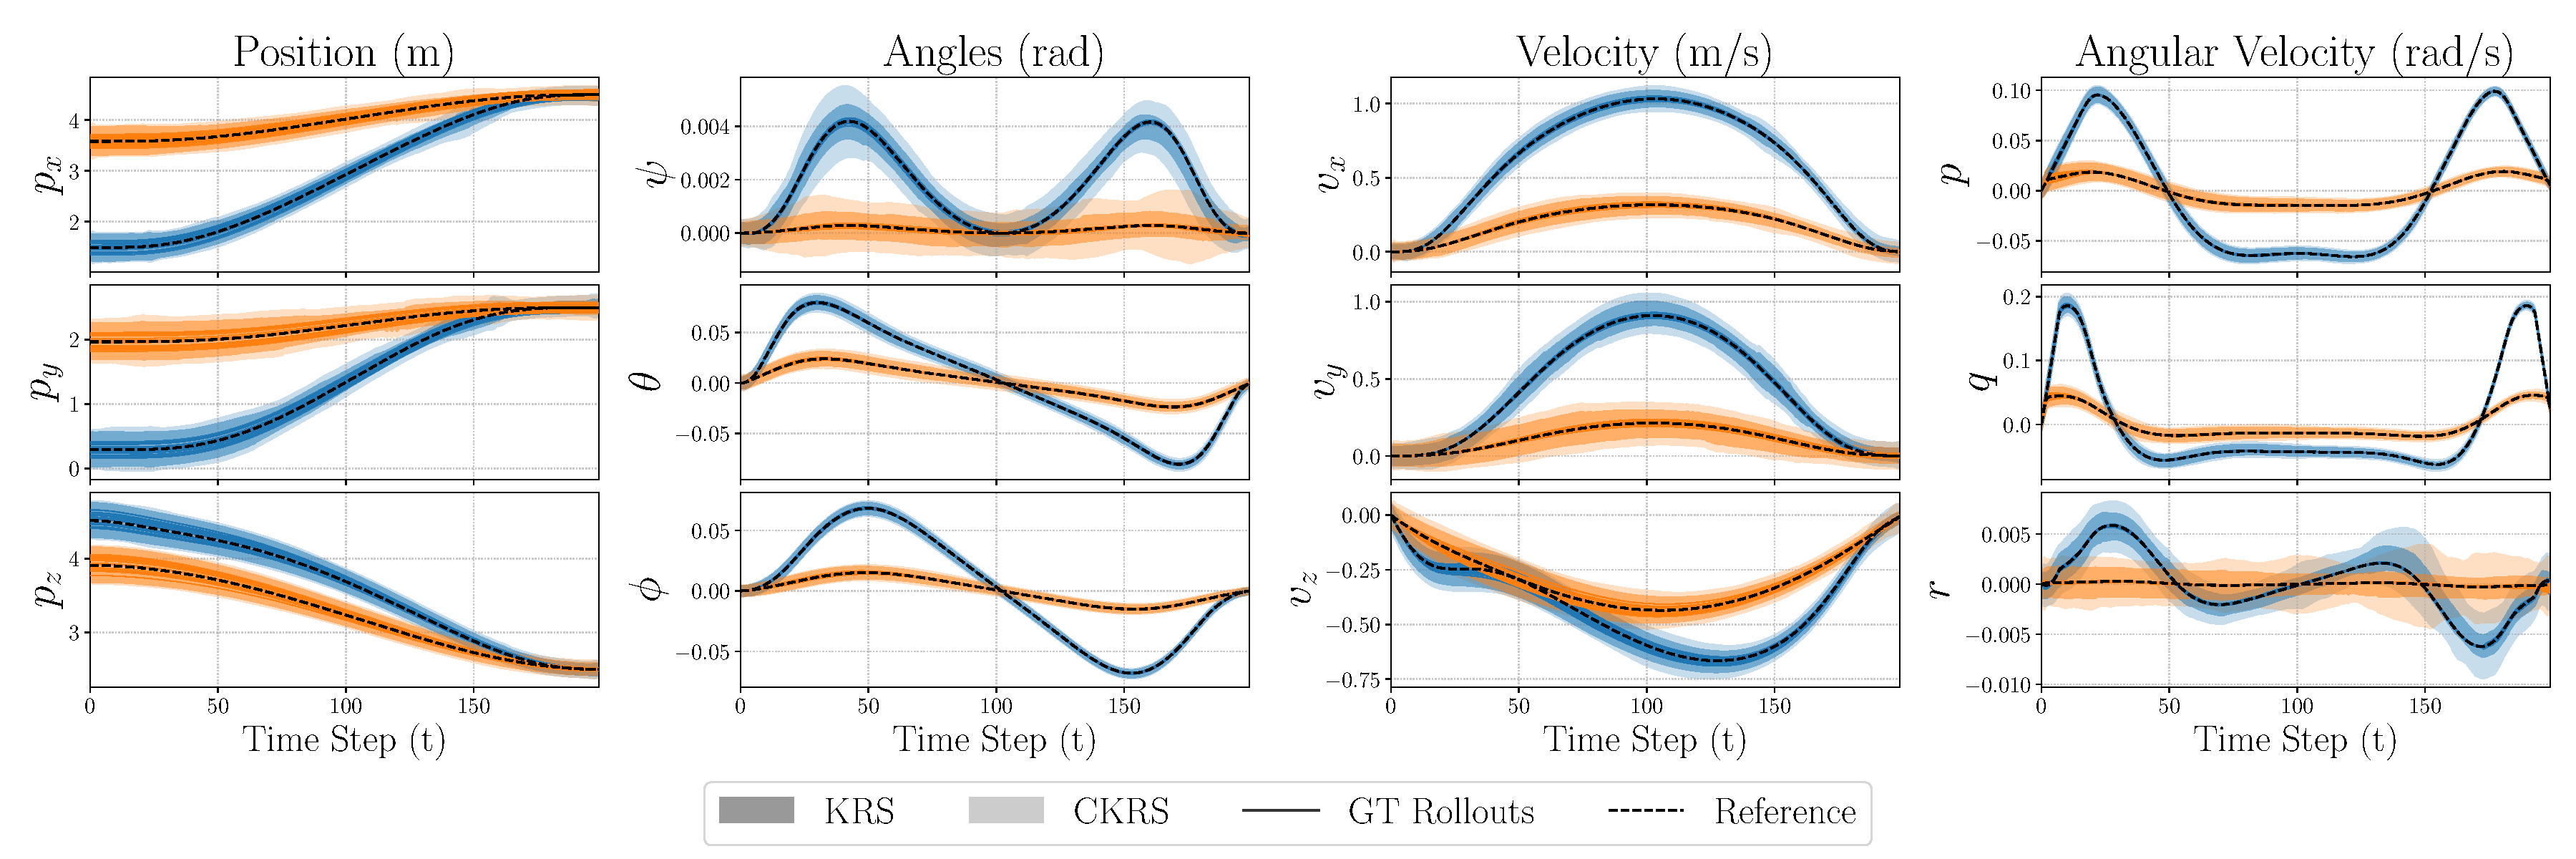
\includegraphics[width=\linewidth]{img/3dquad/3dquad_offline_overlay.pdf}
    \caption{CKRS and KRS (pre-CP) computed for 3D quadcopter, plotted for each dimension.}
    \label{fig:3d_quad}
\end{figure}

\paragraph{MuJoCo: Hopper}
\looseness-1
We evaluate on MuJoCo’s Hopper-v5 \citep{todorov2012mujoco}, a nonlinear, underactuated system with black-box dynamics. A PPO agent (Stable-Baselines3, default hyperparameters) trained for $2\times 10^6$ steps is used as the planner $P$ that generates trajectories for the training dataset. Here, $\enc$ and $\dec$ have 3 hidden layers with 128 neurons each, and $z \in \mathbb{R}^{24}$. Numerical results are in Table~\ref{tab:result_tab} and RSOA slices for a few state dimensions are shown in Fig.~\ref{fig:hopper} (see Fig. \ref{fig:hopper_exp} for all 11 dimensions). This experiment highlights that our approach scales to black-box, high-dimensional contact-rich dynamics while maintaining low runtimes and probabilistic coverage guarantees.

\paragraph{MuJoCo: Customized Swimmer}
\looseness-1
We further assess scalability on a customized MuJoCo Swimmer-v5 \citep{todorov2012mujoco} with extended links, yielding a 28-dimensional state. The planner $P$ is a PPO agent (Stable-Baselines3 MLP) trained for $1\times10^{7}$ steps with modified hyperparameters (LR $1\times10^{-3}$, $\gamma=0.9999$, batch size $512$; others default). Here, $\enc$ and $\dec$ have 3 hidden layers with 128 neurons each, and $z \in \mathbb{R}^{38}$. Numerical results are in Table~\ref{tab:result_tab} and RSOA slices for a few state dimensions are shown in Fig.~\ref{fig:hopper} (see Fig. \ref{fig:swimmer} for all 28 dimensions). This experiment indicates that our approach maintains certified probabilistic safety while tractably computed RSOAs for high-dimensional systems over long horizons for black-box dynamical systems in MuJoCo.
